\documentclass[tikz]{standalone}
\usepackage{fixltx2e}%  http://ctan.org/pkg/fixltx2e

\usepackage[utf8]{inputenx}%  http://ctan.org/pkg/inputenx
% Euler for math | Palatino for rm | Helvetica for ss | Courier for tt
\renewcommand{\rmdefault}{ppl}% rm
\linespread{1.025}% Palatino needs more leading
%\usepackage[scaled]{helvet}% ss //  http://ctan.org/pkg/helvet
%\usepackage{courier}% tt // http://ctan.org/pkg/courier
\usepackage[sc,osf]{mathpazo}
\usepackage[euler-digits,small]{eulervm}  %  http://ctan.org/pkg/eulervm
% a better implementation of the euler package (not in gwTeX)
\normalfont%
\usepackage[T1]{fontenc}%  http://ctan.org/pkg/fontenc
\usepackage{textcomp}%  http://ctan.org/pkg/textcomp

\usepackage{pgfplots}
\pgfplotsset{compat = newest}

\begin{document}
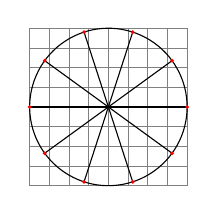
\begin{tikzpicture}
  % drawing unit circle and grid
  \draw[help lines, step = 0.25cm] (-1cm, -1cm) grid (1cm, 1cm);
  \draw[samples = 100, domain = 0:360]
  plot({cos(\x)}, {sin(\x)});
  % fill in roots of unit
  \foreach \k in{0, 2, 4, 6, 8, ..., 18}{
    \draw[thin] (0, 0) -- plot({cos(\k*180/10)}, {sin(\k*180/10)});
    \fill[red] plot({cos(\k*180/10)}, {sin(\k*180/10)})
    circle[radius = 0.025cm];
  }
\end{tikzpicture}
\end{document}

%%% Local Variables:
%%% mode: latex
%%% TeX-master: t
%%% End:
